%% Problema: deve essere grassetto nella ToC e nel titolo del capitolo, ma non grassetto nell'header.
\chapter{Signal event selection}
\label{cap:event_selection}

\section{Prefiltering}
\label{sec:prefilter}
I grafici necessari probabilmente ha senso metterli qui. Magari puoi cambiare il nome in "prefiltering and data characteristics".

\begin{figure}[t]
	\centering
	\begin{subfigure}{.45\textwidth}
		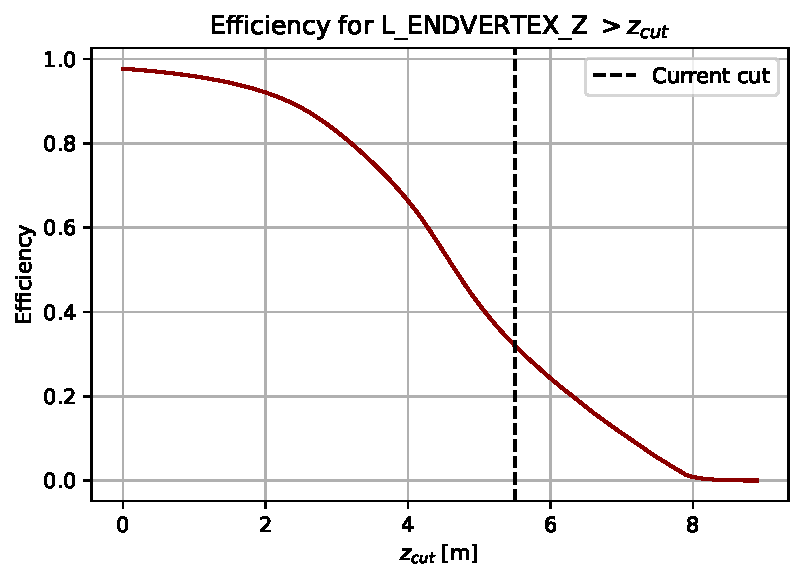
\includegraphics[width=\textwidth]{graphics/04-event_selection/LEVz_left.pdf}
		\caption{}
	\end{subfigure}
	\begin{subfigure}{.45\textwidth}
		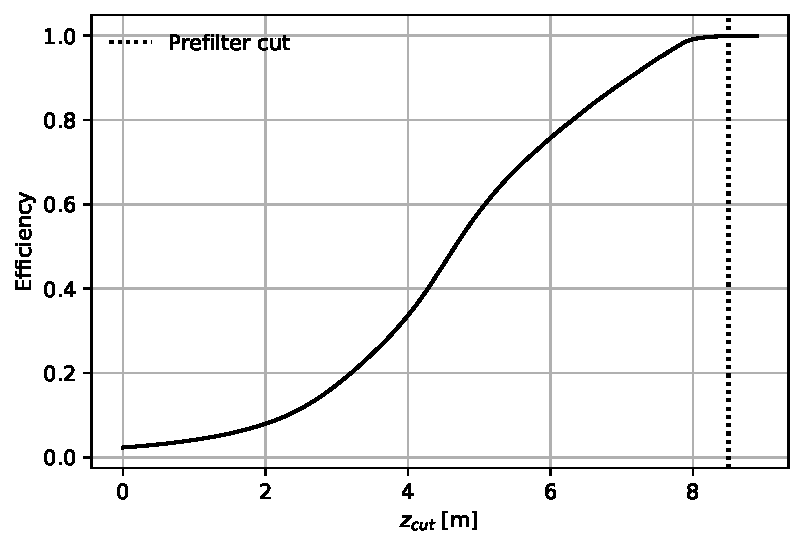
\includegraphics[width=\textwidth]{graphics/04-event_selection/LEVz_right.pdf}
		\caption{}
	\end{subfigure}
	\caption[A and b.]{Boh...}
\end{figure}

\begin{figure}[t]
	\centering
	\begin{subfigure}{.45\textwidth}
		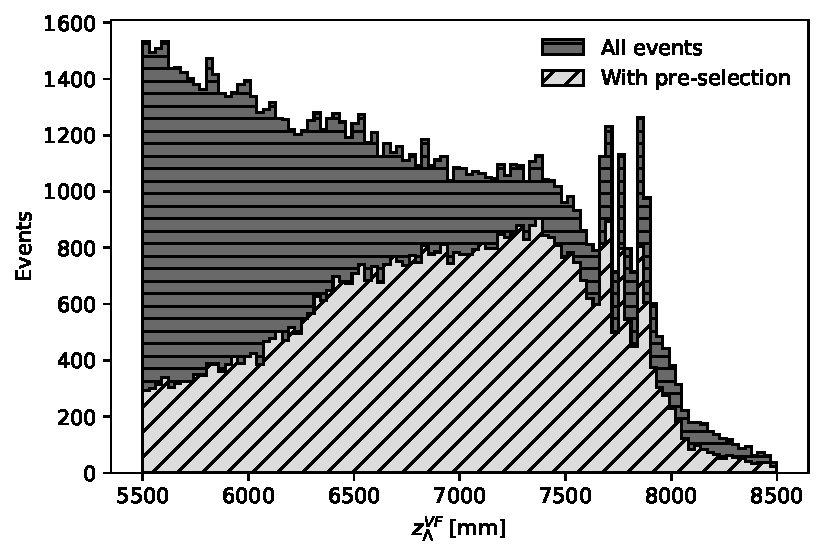
\includegraphics[width=\textwidth]{graphics/04-event_selection/Lambda_endvertex_z.pdf}
		\caption{}
	\end{subfigure}
	\begin{subfigure}{.45\textwidth}
		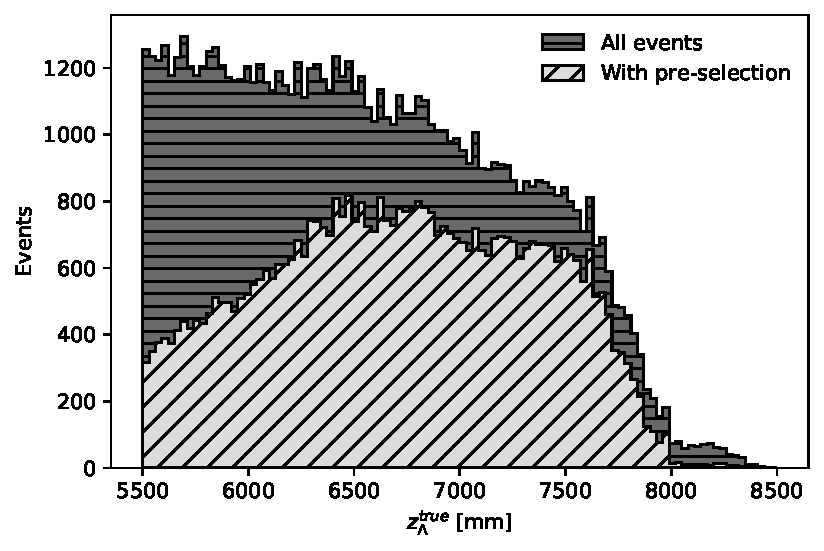
\includegraphics[width=\textwidth]{graphics/04-event_selection/Lambda_endvertex_z_true.pdf}
		\caption{}
	\end{subfigure}
	\caption[Distribution of reconstructed and true $z_\Lambda^\text{vtx}$ in simulated $\Lambda_b^0$ signal events.]{Distribution of reconstructed (\textit{left}) and true (\textit{right}) $z_\Lambda^\text{vtx}$ in simulated $\Lambda_b^0$ signal events, without (\textit{dark grey}) and with (\textit{light grey}) prefiltering.}
\end{figure}

\begin{figure}[t]
	\centering
	\begin{subfigure}{.45\textwidth}
		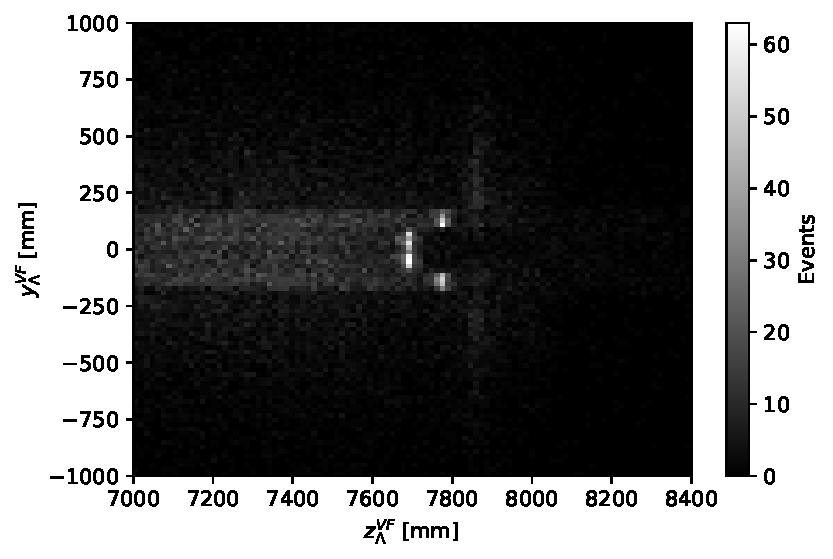
\includegraphics[width=\textwidth]{graphics/04-event_selection/Lambda_endvertex_z_vs_y.pdf}
		\caption{}
	\end{subfigure}
	\begin{subfigure}{.45\textwidth}
		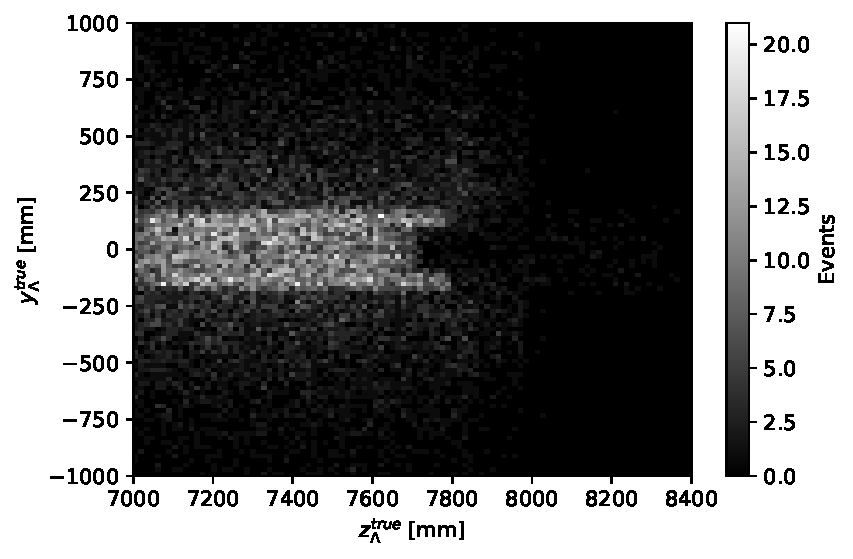
\includegraphics[width=\textwidth]{graphics/04-event_selection/Lambda_endvertex_z_vs_y_true.pdf}
		\caption{}
	\end{subfigure}
	\caption{Event distribution of simulated \lbz signal events as a function of reconstructed (\textit{left}) and true (\textit{right}) $y_\Lambda^\text{vtx}$ and $z_\Lambda^\text{vtx}$.}
\end{figure}

Confronto con Figure \ref{fig:2:t_station_top}.

\subsection{Reconstruction of \texorpdfstring{\lz}{Lambda} decay vertex}
\label{sec:lambda_endvertex_bias}
\begin{figure}[t]
	\centering
	\begin{subfigure}{.45\textwidth}
		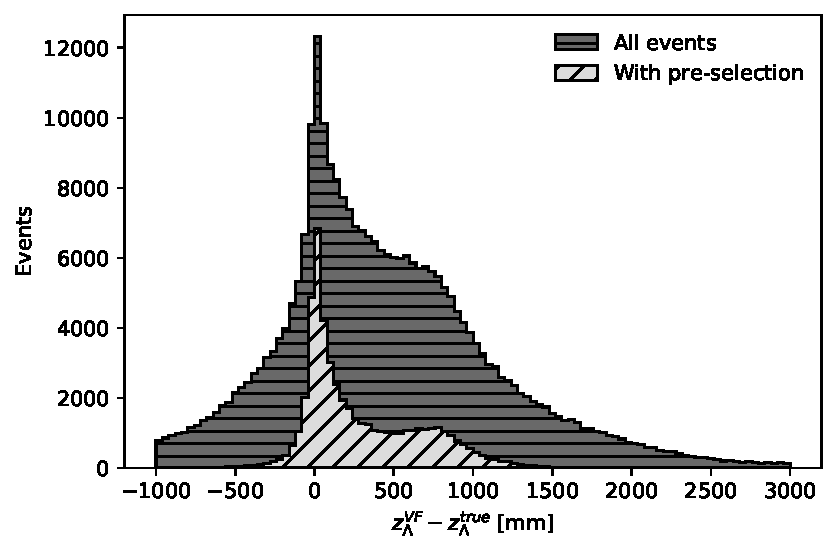
\includegraphics[width=\textwidth]{graphics/04-event_selection/Lambda_endvertex_bias_z.pdf}
		\caption{}
	\end{subfigure}
	\begin{subfigure}{.45\textwidth}
		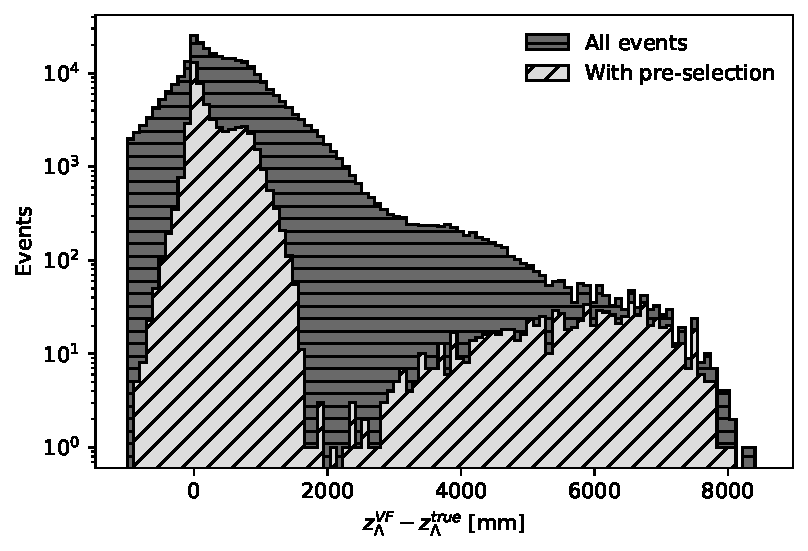
\includegraphics[width=\textwidth]{graphics/04-event_selection/Lambda_endvertex_bias_z_log.pdf}
		\caption{}
	\end{subfigure}
	\caption{Aboh.}
\end{figure}

\begin{figure}[t]
	\centering
	\begin{subfigure}{.45\textwidth}
		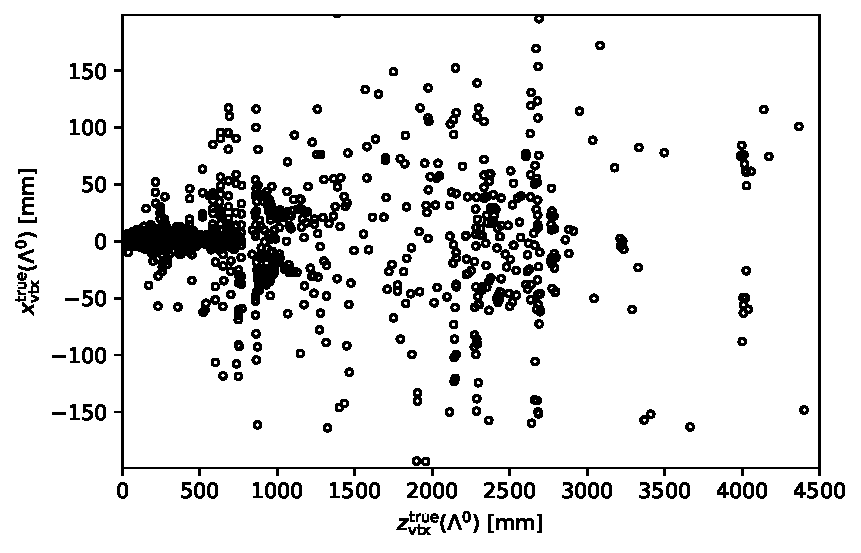
\includegraphics[width=\textwidth]{graphics/04-event_selection/bump_Lambda_true_endvertex_z_vs_x.pdf}
		\caption{}
	\end{subfigure}
	\begin{subfigure}{.45\textwidth}
		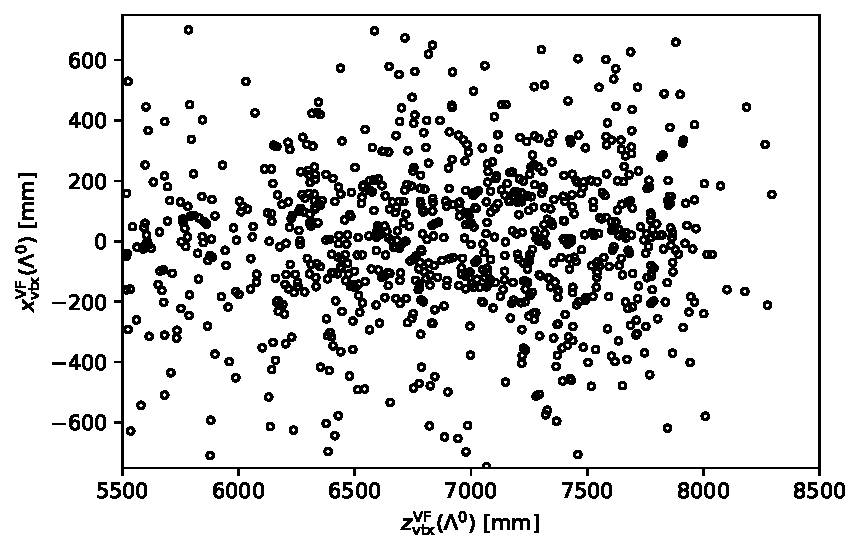
\includegraphics[width=\textwidth]{graphics/04-event_selection/bump_scatter_Lambda_endvertex_z_vs_x.pdf}
		\caption{}
	\end{subfigure}
	\caption[A and b.]{Boh...}
\end{figure}


\begin{figure}[t]
	\centering
	\begin{subfigure}{.45\textwidth}
		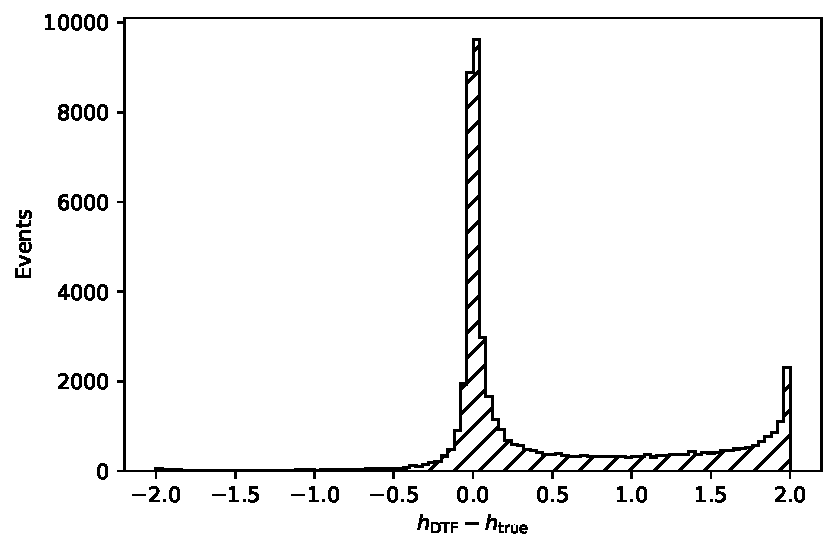
\includegraphics[width=\textwidth]{graphics/04-event_selection/Lambda_horizontality_bias.pdf}
		\caption{}
	\end{subfigure}
	\begin{subfigure}{.45\textwidth}
		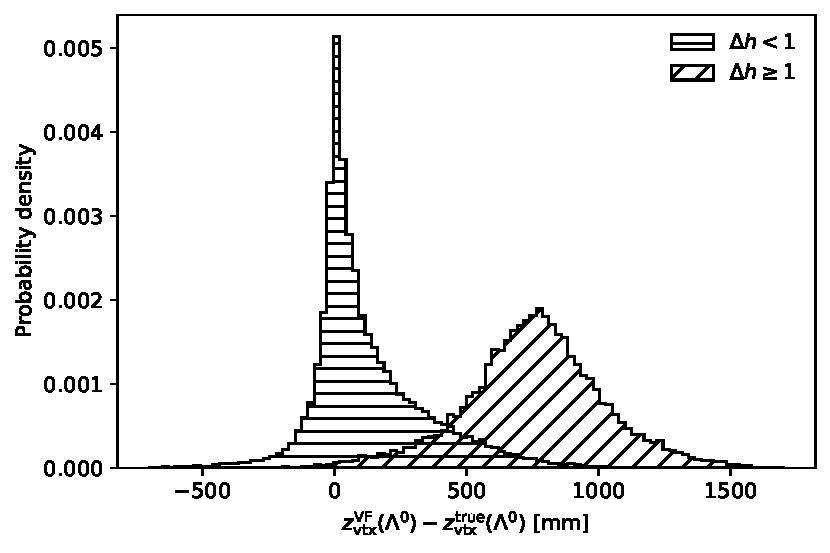
\includegraphics[width=\textwidth]{graphics/04-event_selection/lambda_endvertex_z_bias_vs_horizontality_bias.pdf}
		\caption{}
	\end{subfigure}
	\caption[A and b.]{Boh...}
\end{figure}

Qui devi menzionare l'orizzontalità, perché vi faccio riferimento nel Cap. 3. Devi dire che c'è il problema con grafico.

\section{Physical background veto}
\label{sec:B0_veto}
\begin{figure}[t]
	\centering
	\begin{subfigure}{.45\textwidth}
		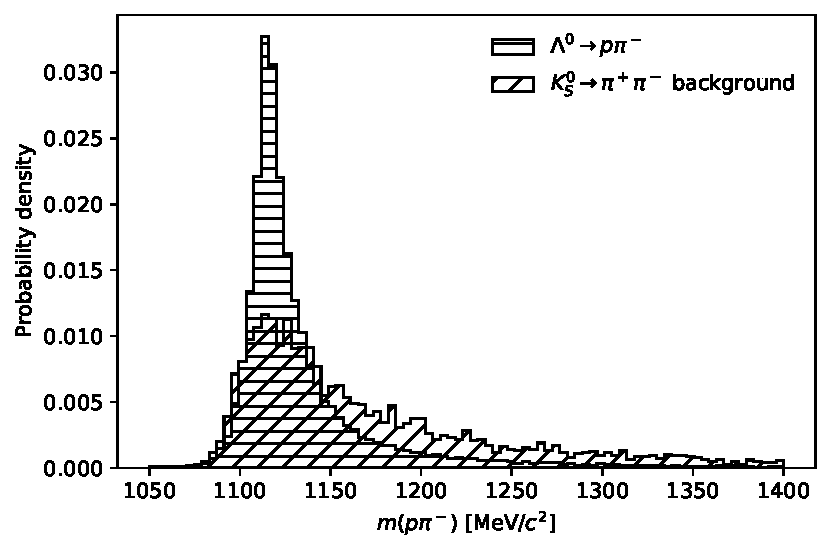
\includegraphics[width=\textwidth]{graphics/04-event_selection/phys_bkg_lambda_comparison.pdf}
		\caption{}
	\end{subfigure}
	\begin{subfigure}{.45\textwidth}
		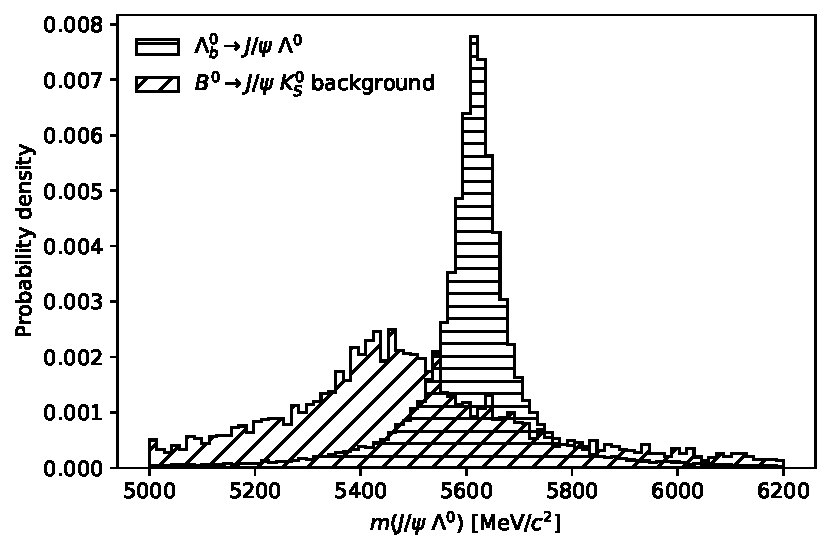
\includegraphics[width=\textwidth]{graphics/04-event_selection/phys_bkg_lambdab_comparison.pdf}
		\caption{}
	\end{subfigure}
	\caption[Comparison of simulated $m(p\pi^-)$ \textit{(a)} and $m(J/\psi~\Lambda^0)$ distributions for simulated \demonstratorshort signal and \physbkgshort physical background with proton mass hypothesis.]{Comparison of simulated $m(p\pi^-)$ \textit{(a)} and $m(J/\psi~\Lambda^0)$ \textit{(b)} distributions: \demonstratorshort signal is labeled by horizontal hatching, \physbkgshort physical background with $\pi^+ \rightarrow p$ mass hypothesis by diagonal hatching.}
\end{figure}

\begin{figure}[t]
	\centering
	\begin{subfigure}{.45\textwidth}
		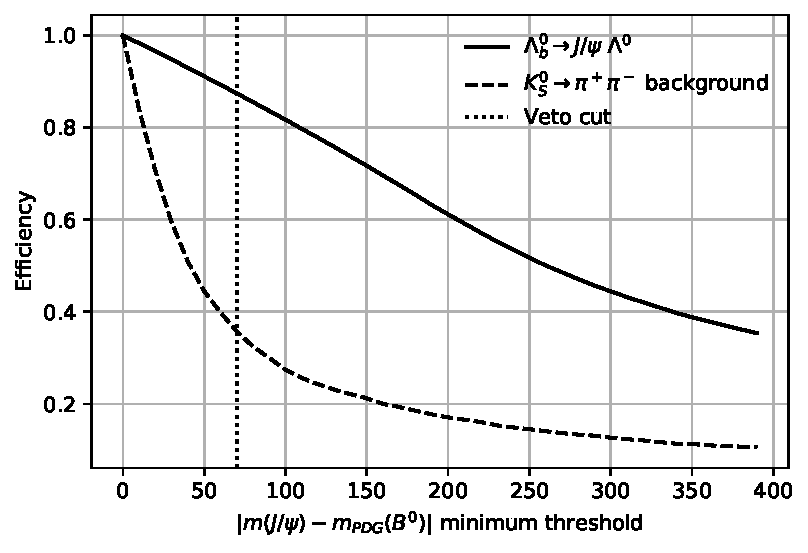
\includegraphics[height=.2\textheight]{graphics/04-event_selection/phys_veto_efficiencies.pdf}
		\caption{}
	\end{subfigure}
	\begin{subfigure}{.45\textwidth}
		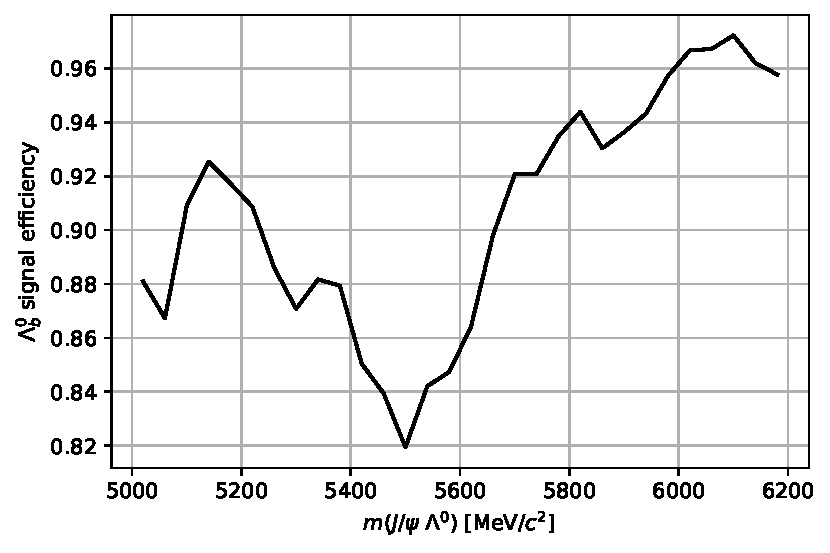
\includegraphics[height=.2\textheight]{graphics/04-event_selection/phys_veto_sig_efficiencies_per_bin.pdf}
		\caption{}
	\end{subfigure}
	\caption[Efficiency of the physical background veto as a function of the invariant mass discrepancy threshold and of $J/\psi~\Lambda^0$ invariant mass bins.]{\textit{(a)} Efficiency of physical background veto as a function of the invariant mass discrepancy threshold on simulated signal (\demonstratorshort, solid) and background (\physbkgshort with proton mass hypothesis, dashed) events. Chosen threshold marked by dotted line. \textit{(b)} Efficiency of the veto on different $m(J/\psi~\Lambda^0)$ bins for \demonstratorshort signal events).}
\end{figure}

\section{HBDT classifier}
\label{sec:HBDT}

\subsection{Training data}

\begin{figure}[t]
	\centering
	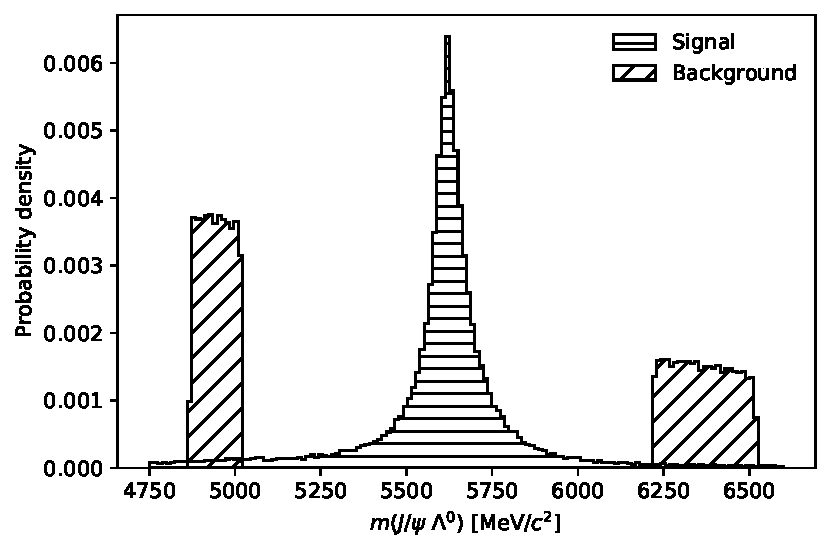
\includegraphics[width=.6\textwidth]{graphics/04-event_selection/sig_bkg_distribution_balance.pdf}
	\caption{Signal (\textit{horizontal hatching}) and background (\textit{diagonal hatching}) data samples used for training the HBDT classifier. Test samples are taken from the same pool in 1:9 ratio.}
	\label{fig:4:HBDT_training_data}
\end{figure}

\subsection{Hyperparameter optimization and performance test}
\begin{figure}[t]
	\centering
	\begin{subfigure}{.45\textwidth}
		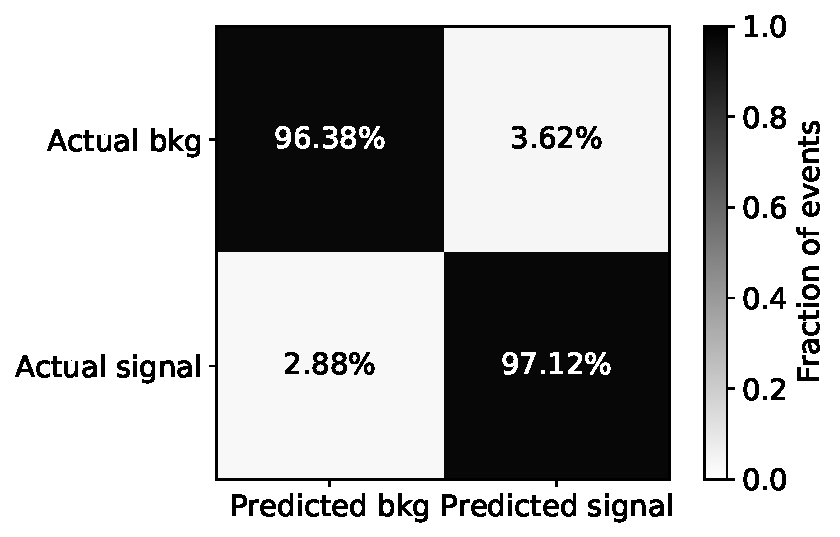
\includegraphics[width=\textwidth]{graphics/04-event_selection/confmatrix_train.pdf}
		\caption{}
	\end{subfigure}
	\begin{subfigure}{.45\textwidth}
		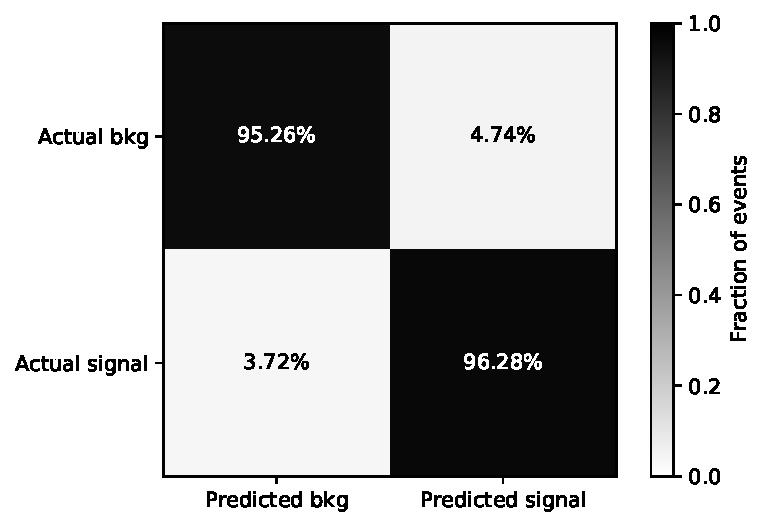
\includegraphics[width=\textwidth]{graphics/04-event_selection/confmatrix_test.pdf}
		\caption{}
	\end{subfigure}
	\caption{Confusion matrices visualizing the performance of the HBDT classifier on training \textit{(a)} and testing \textit{(b)} data samples. Percentages and chromatic scale are normalized to the true event classification: for instance, the top left and top right quadrants of a matrix represent the fraction of true background events reconstructed as background or signal, respectively. Binary classification uses an illustrative response threshold $s_\text{thres} = 0.5$.}
\end{figure}

\begin{figure}[t]
	\centering
	\begin{subfigure}{.45\textwidth}
		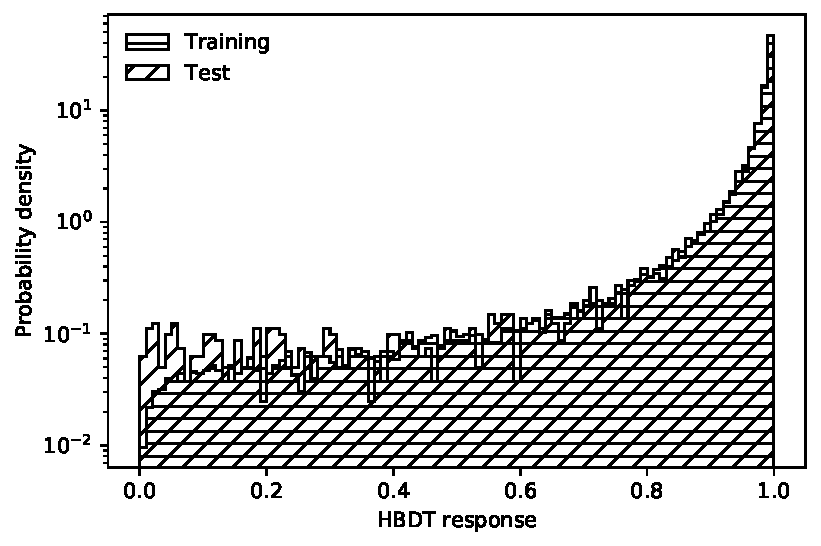
\includegraphics[width=\textwidth]{graphics/04-event_selection/sig_train_vs_test.pdf}
		\caption{}
	\end{subfigure}
	\begin{subfigure}{.45\textwidth}
		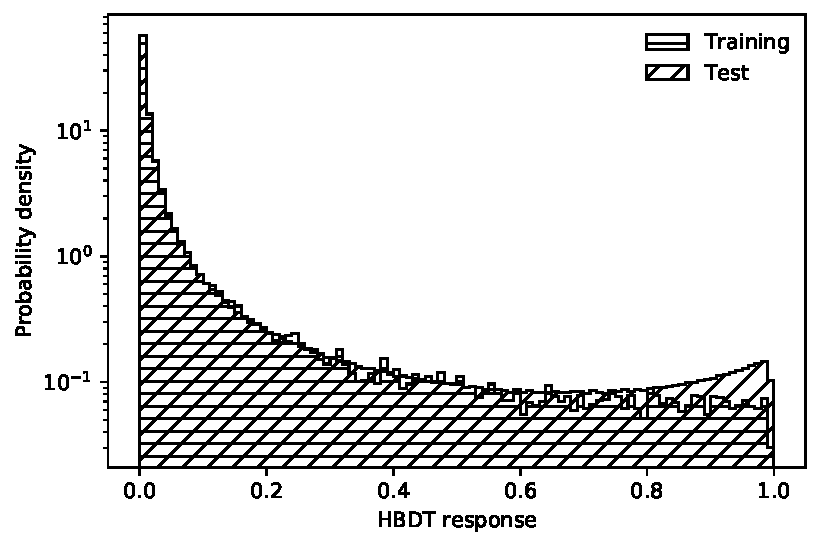
\includegraphics[width=\textwidth]{graphics/04-event_selection/bkg_train_vs_test.pdf}
		\caption{}
	\end{subfigure}
	\caption{Response distribution of the HBDT classifier on signal \textit{(a)} and background \textit{(b)} events. The training sample is represented by horizontal hatching, the test sample by diagonal hatching.}
\end{figure}

\begin{figure}
	\centering
	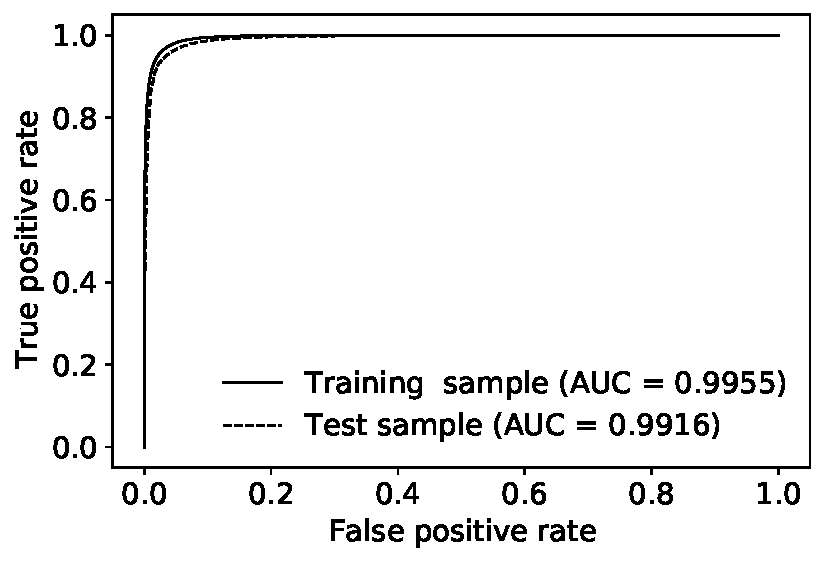
\includegraphics[width=.6\textwidth]{graphics/04-event_selection/roc.pdf}
	\caption{Receiving operating characteristic (ROC) curve for the HBDT classifier on training (\textit{solid}) and test (\textit{dashed}) samples. The legend includes the area-under-curve (AUC) score.}
\end{figure}

\subsection{Threshold optimization}

\begin{figure}
	\centering
	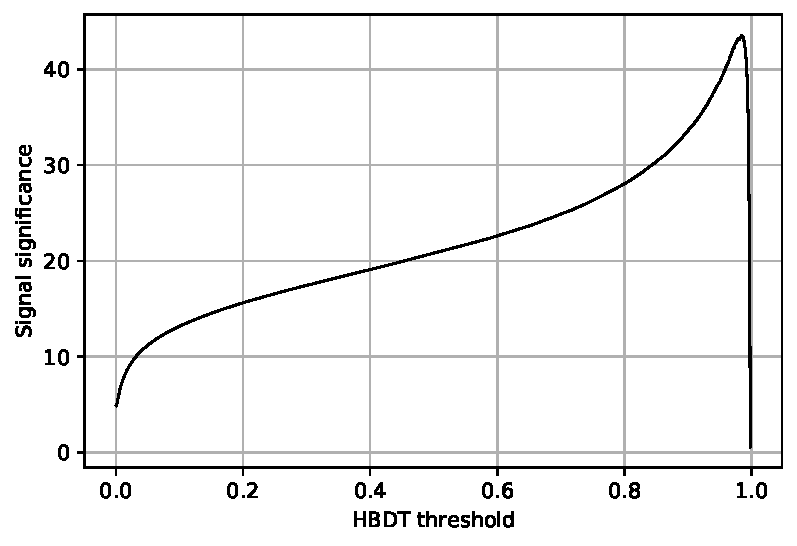
\includegraphics[width=.6\textwidth]{graphics/04-event_selection/HBDT_signal_significance.pdf}
	\caption{Projected \demonstratorshort signal significance over background as a function of the HBDT response threshold used for selection.}
\end{figure}

\section{Performance on data}
Gli invariant mass fits, essenzialmente.

\begin{figure}[t]
	\centering
	\begin{subfigure}{.45\textwidth}
		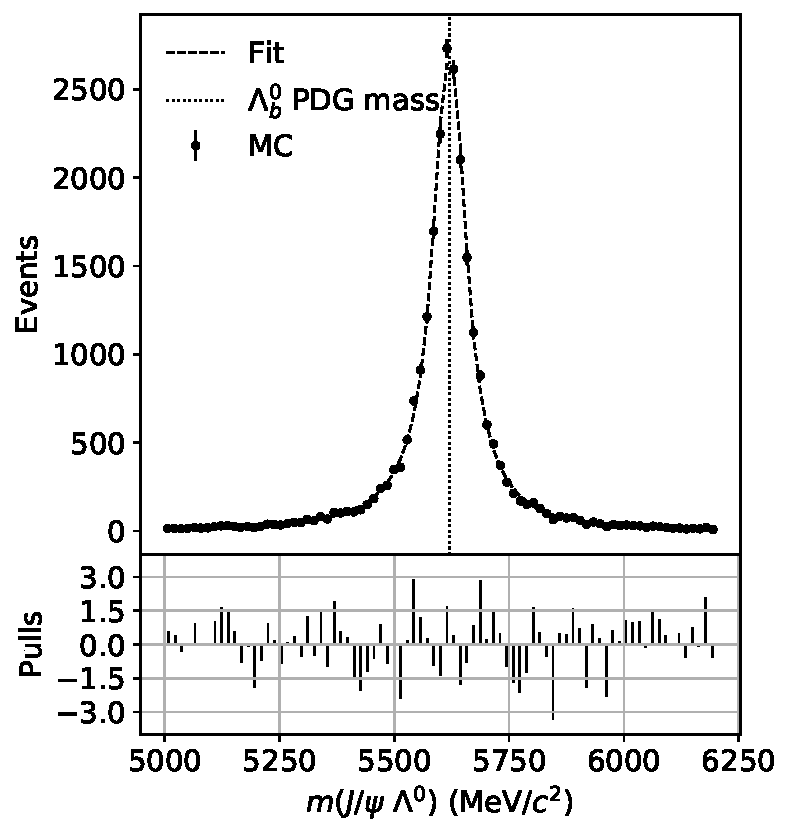
\includegraphics[width=\textwidth]{graphics/04-event_selection/MC_lambdab_hard_fit.pdf}
		\caption{}
	\end{subfigure}
	\begin{subfigure}{.45\textwidth}
		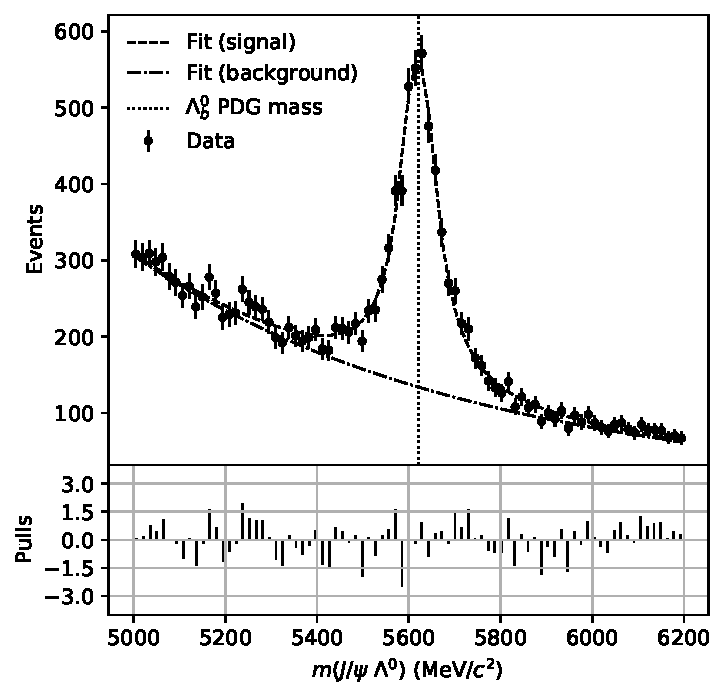
\includegraphics[width=\textwidth]{graphics/04-event_selection/data_lambdab_hard_fit.pdf}
		\caption{}
	\end{subfigure}
	\caption{Fitted $m(J/\psi~\Lambda^0)$ invariant mass distributions for simulated \demonstratorshort events \textit{(a)} and Run 2 data \textit{(b)} after all selection steps. Signal fit function is \textit{dashed}, background fit function in \textit{(b)} is \textit{dash-dotted}. The current best measurement for $\Lambda_b^0$ mass is marked by the \textit{dotted vertical line}. Fit pulls (data-fit discrepancy divided by uncertainty) are shown below the main plots.}
\end{figure}
